% !TeX program = lualatex
\documentclass[UTF8,zihao=-4,fontset=fandol]{ctexart}
\usepackage[a4paper,top=2.15cm,bottom=2.3cm,left=2.3cm,right=2.3cm]{geometry}
\usepackage{amsmath,amssymb,bm,booktabs,array,graphicx,caption,float,enumitem,longtable}
\usepackage{fancyhdr,microtype,setspace,url}
\graphicspath{{output/pdf/sun2018_zh_figures/}{sun2018_zh_figures/}}
\setstretch{1.20}
\setlength{\parindent}{2em}
\setlength{\parskip}{0.16em}
\setlength{\headheight}{14pt}
\captionsetup{font=small,labelsep=quad}
\pagestyle{fancy}
\fancyhf{}
\fancyhead[L]{\small 铝电解槽阳极下气泡生长与聚并的多尺度数学模型}
\fancyhead[R]{\small Sun 等（2018）}
\fancyfoot[C]{\thepage}
\renewcommand{\headrulewidth}{0.4pt}
\ctexset{
 section={format=\large\bfseries,name={},number=\Roman{section}.,aftername=\quad},
 subsection={format=\normalsize\bfseries,name={},number=\Alph{subsection}.,aftername=\quad}
}
\newcommand{\vect}[1]{\bm{#1}}
\newcommand{\dd}{\mathrm{d}}
\title{\bfseries 铝电解槽阳极下气泡生长与聚并的多尺度数学模型\\
\large A Multi-scale Mathematical Model of Growth and Coalescence of Bubbles\\
Beneath the Anode in an Aluminum Reduction Cell}
\author{孙美佳（Meijia Sun）\textsuperscript{a,b}，李宝宽（Baokuan Li）\textsuperscript{a,*}，\\
李林珉（Linmin Li）\textsuperscript{c}\\[0.7em]
\small\textsuperscript{a}东北大学冶金学院，辽宁沈阳 110819\\
\small\textsuperscript{b}复杂有色金属资源清洁利用国家重点实验室，云南昆明 650093\\
\small\textsuperscript{c}河海大学能源与电气学院，江苏南京 210098\\
\small\textsuperscript{*}\texttt{libk@smm.neu.edu.cn}}
\date{\small \emph{Metallurgical and Materials Transactions B}（2018）\\
\url{https://doi.org/10.1007/s11663-018-1311-y}}

\begin{document}
\maketitle
\thispagestyle{empty}
\begin{center}\small\itshape 中文翻译稿；公式编号、图号、表号及章节结构与原文对应。\end{center}

\begin{abstract}
由于铝电解槽内所涉及的长度尺度跨度很大，气泡形态建模具有较大挑战性。
本文建立了一个三维多尺度数学模型，用于认识阳极下气泡的成核、生长和聚并过程，并研究气泡由微观尺度向宏观尺度的转化。
在拉格朗日参考系下采用离散气泡模型（DBM）研究微气泡运动；通过用户自定义函数实现离散微气泡向大气泡的转化，而大气泡则由流体体积法（VOF）完整解析。
离散气泡与连续流体之间通过相间动量交换实现双向耦合。
模型包含三类气泡聚并：微气泡间聚并由 DBM 处理；大气泡吞并微气泡由离散-连续转化模型处理；大气泡间聚并由 VOF 方法处理。
数值结果表明，气泡覆盖率和气泡层厚度与文献实验数据吻合良好。当气泡沿阳极底面伸展时，其厚度停止增加，稳定在 4.0--4.5 mm；同时可在阳极下观察到两个不对称的厚头部。气泡释放频率随电流密度升高而增大。
\end{abstract}

\noindent\textbf{关键词：}铝电解槽；多尺度气泡；离散气泡模型；流体体积法；离散-连续转化；气泡聚并

\section{引言}

在现代铝电解槽中（图~\ref{fig:cell}），直流电依次通过阳极、熔融电解质（电解质熔体）和铝液层，并流向最近的阴极导电棒。
氧化铝在约 1223 K 的高温下加入电解质层并溶解，随后发生电化学反应。阳极下首先生成微小气泡，继而通过传质和聚并长大；较大的气泡以缓慢蠕动方式离开成核位置，最终移向阳极边缘并从阳极底面逸出。

气泡既有积极作用，也有消极作用：它能强化氧化铝在电解质中的混合与溶解，促进电解质与侧壁之间的传热；但也会减小电解质与阳极的接触面积，降低电化学反应速率，增大阳极-阴极距离（ACD）内的电阻和电压降，并因气泡脱离造成电解质扰动，诱发磁流体动力学（MHD）不稳定性。因此，要充分利用气泡的有利作用并尽量削弱其不利影响，就必须深入认识电解质中的气泡动力学。

\begin{figure}[H]\centering
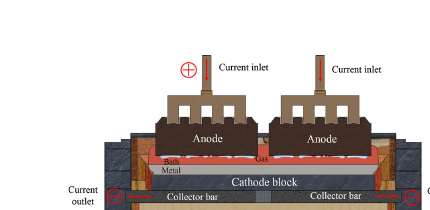
\includegraphics[width=0.72\textwidth]{fig01.png}
\caption{铝电解槽示意图。}
\label{fig:cell}
\end{figure}

铝电解槽内部温度高、运行环境恶劣，普通测量手段难以直接观测气泡运动。为此，研究者开展了大量空气-水物理模拟实验\([1\text{-}9]\)。Fortin 等\([1]\)采用全尺寸水模型研究气泡行为，发现提高电流密度会增大气泡尺寸、气泡层厚度和气泡速度；提高电解质流速则减小气泡尺寸和气体覆盖率，但提高气泡速度及释放频率。V\'ekony 和 Kiss\([2]\)在含两个倾斜阳极的实尺寸空气-水电解模型中发现，由于 Fortin 气泡的存在，最大气泡高度可达 2 cm。Simonsen 等\([3]\)研究了倾斜表面下气泡的聚并和运动，并通过添加 NaCl 提高表面张力；NaCl 溶液中的气泡尺寸大于纯水，体系还表现出接近自组织的状态。

Alam 等\([4]\)以硫酸铜溶液为电解质，研究水平阳极下气泡的形成、聚并和运动。Perron 等\([5,6]\)指出，气泡终端速度随气泡体积和表面倾角增大而上升。Kiss 等\([7]\)分析了朝下固体表面下方气泡离开与脱离的机制，表明表面力、浮力、流动力和液体惯性力之间的相互作用会导致复杂的气泡形态演化。Das 等\([8,9]\)发现，降低表面张力会减小气泡厚度和滞留时间，而气泡脱离与滑移主要由浮力、曳力和表面张力之间的平衡决定。

然而，空气-水体系不能完全代表实际铝电解槽内的 CO$_2$-冰晶石体系。Zhao 等\([10]\)基于 CFD-VOF 模型指出，与水中的空气泡相比，冰晶石熔体中的 CO$_2$ 气泡厚度更小、展弦比更大、滑移速度更高。针对更接近工业环境的 CO$_2$-冰晶石体系，已有许多研究\([11\text{-}20]\)。Xue 和 Oye\([11]\)利用透明铝电解实验研究气泡生成、聚并、生长、脱离及其与槽电压波动的耦合关系：小幅电压波动与气泡聚并和生长有关，而较大幅度波动与气泡脱离有关。Cassayre 等\([12]\)发现，析氧阳极逸出的气泡直径远小于石墨阳极；电解质润湿性良好时易形成微小气泡。Zhao 等\([13,14]\)的透明铝电解槽实验进一步确认，润湿性是空气-水体系和 CO$_2$-冰晶石体系气泡动力学差异的主导因素，并展示了气泡生长期间的多种聚并形式。

高温小型电解槽有助于研究气泡行为，但由于设备成本高，其阳极尺寸远小于工业阳极。数值模拟因此逐渐成为重要替代工具。Kiss\([21]\)基于有限元法建立单气泡生长模型，指出生长速率主要受扩散阻力和阳极固体内部储气能力影响。Perron 等\([22,23]\)发现气泡形态对相对电阻的影响较小。VOF 方法\([24,25]\)适合描述阳极下被压扁的大气泡，但解析微小气泡界面需要大量网格，计算代价很高。欧拉-欧拉方法和群体平衡模型（PBM）\([26\text{-}34]\)能描述气泡尺寸分布，但不能跟踪单个气泡轨迹，也不能解析气泡界面。拉格朗日离散气泡模型（DBM）\([35]\)可以跟踪轨迹并具有直接物理解释，但通常把气泡视为球形，无法描述大气泡变形。

因此，多尺度气泡共存是数值模拟的关键难题。本文提出一种新的微气泡到大气泡转化模型：用 DBM 跟踪离散微气泡，用 VOF 捕捉大气泡-电解质界面；依据法拉第定律计算离散气泡生长，以 DBM 描述微气泡碰撞聚并，通过 DBM 与 VOF 耦合处理变形大气泡吞并离散气泡，并用 VOF 完整解析大气泡之间的聚并。最后将结果与已有实验数据比较以验证模型。

\section{模型构建}

为在合理计算时间内描述铝电解槽内复杂的气泡行为与输运过程，作如下假设：
\begin{enumerate}[label=\arabic*.]
\item 气泡和电解质均为不可压缩牛顿流体；
\item 忽略阳极与电解质之间的电化学反应过程本身；
\item 不考虑温度场；
\item 不考虑阳极表面粗糙度和储气孔穴，气泡在阳极表面均匀成核。
\end{enumerate}

\subsection{微气泡离散气泡模型}

DBM\([36\text{-}38]\)适合跟踪尺寸较小、近似球形且离散分布的气泡，并可考虑聚并。对浸没在液体中的球形气泡进行受力平衡，在拉格朗日坐标下由牛顿运动定律得到
\begin{align}
m_b\frac{\dd\vect u_b}{\dd t}&=\vect F_b+\vect F_d+\vect F_{\mathrm{vir}}+\vect F_p, \tag{1}\\
\frac{\dd m_b}{\dd t}&=\frac{\rho_b RTA}{4NF p_1^2}I. \tag{2}
\end{align}
式中，气泡质量由下一节的气泡生长模型确定。浮力与重力的合力为
\begin{equation}
\vect F_b=m_b\frac{\vect g(\rho_b-\rho)}{\rho_b}. \tag{3}
\end{equation}
曳力为
\begin{equation}
\vect F_d=\frac{3}{4}\rho V_b\frac{C_D}{d_b}
\left|\vect u-\vect u_b\right|(\vect u-\vect u_b), \tag{4}
\end{equation}
其中球形气泡曳力系数 $C_D$ 采用文献\([39]\)的球形曳力定律。液体中气泡的虚质量力\([40,41]\)为
\begin{equation}
\vect F_{\mathrm{vir}}=\frac{1}{2}\rho V_b\frac{\dd}{\dd t}(\vect u-\vect u_b), \tag{5}
\end{equation}
压力梯度力为
\begin{equation}
\vect F_p=\rho V_b(\vect u_b\cdot\nabla)\vect u. \tag{6}
\end{equation}

\subsection{微气泡生长}

典型 Hall-H\'eroult 电解槽在约 1223 K 下工作。氧化铝溶解于熔融电解质后，电极反应可简写为
\[
\text{阴极：}\quad \mathrm{Al^{3+}+3e^-\rightarrow Al},
\qquad
\text{阳极：}\quad \mathrm{C+2O^{2-}-4e^-\rightarrow CO_2}.
\]
因此每生成 1 mol Al 对应生成 $3/4$ mol CO$_2$。由法拉第定律，CO$_2$ 的物质的量为
\begin{equation}
n_{\mathrm{CO_2}}=\frac{It}{3F}\frac{3}{4}=\frac{It}{4F}. \tag{7}
\end{equation}
依据理想气体方程，CO$_2$ 体积为
\begin{equation}
V_{\mathrm{CO_2}}=\frac{IRT}{4Fp_1}t, \tag{8}
\end{equation}
而电解质内气泡压力（图~\ref{fig:pressure}）为
\begin{equation}
p_1=p_0+\rho_l gH+\frac{2\sigma}{r}. \tag{9}
\end{equation}
阳极底面的气体生成量为
\begin{equation}
q=\frac{V_{\mathrm{CO_2}}}{A}=\frac{IRT}{4Fp_1A}t. \tag{10}
\end{equation}

\begin{figure}[H]\centering
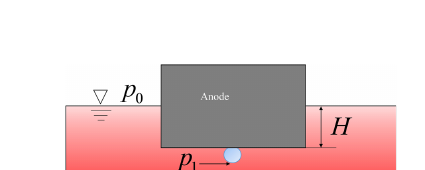
\includegraphics[width=0.62\textwidth]{fig02.png}
\caption{气泡压力示意图。}
\label{fig:pressure}
\end{figure}

实验观察\([11,14]\)表明，阳极底面的初生小气泡近似半球或完整球体，其半径可写为
\begin{equation}
r=\sqrt[3]{\frac{3RTA}{16N\pi Fp_1}It}, \tag{11}
\end{equation}
即
\begin{equation}
r\propto\sqrt[3]{It}. \tag{12}
\end{equation}
式中，$R$ 为摩尔气体常数，$T$ 为温度，$A$ 为阳极底面积，$N$ 为气泡总数。该模型给出气泡体积随电流和时间增加的规律，只适用于成核后的初始球形生长阶段；大气泡因受力不平衡而发生变形，不能继续按球形规律生长。成核位置机理不在本文讨论范围内。

\subsection{微气泡聚并}

依据 O'Rourke 算法\([36,38,42]\)，把半径较大的气泡称为捕集气泡，较小者称为小气泡。当小气泡穿过以捕集气泡为中心、面积为 $\pi(r_1+r_2)^2$ 的圆形碰撞截面时，可能发生碰撞。碰撞概率为
\begin{equation}
P=\frac{\pi(r_1+r_2)^2|\vect u_{\mathrm{rel}}|\Delta t}{V_{\mathrm{cell}}}. \tag{13}
\end{equation}
实际碰撞次数 $N_c$ 服从泊松分布：
\begin{equation}
P(N_c)=\frac{e^{-\bar N}\bar N^{N_c}}{N_c!}, \tag{14}
\end{equation}
其中期望碰撞数为 $\bar N=N_1P$，$N_1$ 为小气泡数。

为判断两气泡碰撞还是回弹，首先生成随机数 $x\in(0,1)$；仅当 $x>P(0)$ 时发生碰撞\([43]\)。再生成随机数 $y\in(0,1)$，实际碰撞偏心距为
\begin{equation}
b=(r_1+r_2)\sqrt{y}. \tag{15}
\end{equation}
若 $b<b_{\mathrm{crit}}$，碰撞结果为聚并。临界偏心距为
\begin{equation}
b_{\mathrm{crit}}=(r_1+r_2)
\sqrt{\min\!\left(1.0,\frac{2.4f}{We}\right)}, \tag{16}
\end{equation}
其中
\begin{align}
f\!\left(\frac{r_1}{r_2}\right)&=
\left(\frac{r_1}{r_2}\right)^3-2.4\left(\frac{r_1}{r_2}\right)^2
+2.7\left(\frac{r_1}{r_2}\right), \tag{17}\\
We&=\frac{\rho_b|\vect u_{\mathrm{rel}}|^2\bar d}{\sigma}. \tag{18}
\end{align}
$\bar d$ 为两气泡直径的算术平均值。聚并后，大气泡吞并小气泡，按质量和动量守恒更新：
\begin{align}
m_1'&=m_1+m_2, \tag{19}\\
m_1'\vect u_b'&=m_1\vect u_{b1}+m_2\vect u_{b2}. \tag{20}
\end{align}
若 $b\ge b_{\mathrm{crit}}$，则发生回弹。气泡质量不变，速度更新为
\begin{align}
\vect u_{b1}'&=\frac{m_1\vect u_{b1}+m_2\vect u_{b2}}{m_1+m_2}
+\frac{m_2(\vect u_{b1}-\vect u_{b2})}{m_1+m_2}
\frac{b-b_{\mathrm{crit}}}{r_1+r_2-b_{\mathrm{crit}}}, \tag{21}\\
\vect u_{b2}'&=\frac{m_1\vect u_{b1}+m_2\vect u_{b2}}{m_1+m_2}
-\frac{m_1(\vect u_{b1}-\vect u_{b2})}{m_1+m_2}
\frac{b-b_{\mathrm{crit}}}{r_1+r_2-b_{\mathrm{crit}}}. \tag{22}
\end{align}

\subsection{大变形气泡的 VOF 方法}

VOF 方法\([44]\)通过求解体积分数输运方程捕捉大变形气泡表面：
\begin{equation}
\frac{\partial\alpha}{\partial t}+\nabla\cdot(\alpha\vect u)=0. \tag{23}
\end{equation}
流场由连续方程和一组共享的动量方程描述\([45]\)：
\begin{align}
\frac{\partial\rho}{\partial t}+\nabla\cdot(\rho\vect u)&=S_1+S_2, \tag{24}\\
\frac{\partial(\rho\vect u)}{\partial t}+\nabla\cdot(\rho\vect u\vect u)&=
-\nabla p+\nabla\cdot\left[\mu\left(\nabla\vect u+\nabla\vect u^{T}\right)\right]
+\vect F_{\mathrm{me}}+\vect F_s. \tag{25}
\end{align}
混合物密度和黏度分别为
\begin{align}
\rho&=\alpha\rho_l+(1-\alpha)\rho_g, \tag{26}\\
\mu&=\alpha\mu_l+(1-\alpha)\mu_g. \tag{27}
\end{align}
式中 $S_1$、$S_2$ 是微气泡转化为解析气泡时引入的质量源项。拉格朗日离散气泡与欧拉连续液相之间通过动量交换项 $\vect F_{\mathrm{me}}$ 双向耦合：
\begin{equation}
\vect F_{\mathrm{me}}=
\left\{\frac{3}{4}\rho V_b\frac{C_D}{d_b}|\vect u-\vect u_b|(\vect u-\vect u_b)
+\frac{1}{2}\rho V_b\frac{\dd}{\dd t}(\vect u-\vect u_b)
+\rho V_b(\vect u_b\cdot\nabla)\vect u\right\}\Delta t. \tag{28}
\end{equation}
表面张力采用 Brackbill\([46]\)提出的连续表面力（CSF）模型：
\begin{align}
\vect F_s&=\sigma_{ij}\kappa\nabla\alpha, \tag{29}\\
\kappa&=-\nabla\cdot\left(\frac{\nabla\alpha}{|\nabla\alpha|}\right). \tag{30}
\end{align}

\subsection{离散-连续转化}

气泡早期尺寸小且近似球形，适合在拉格朗日参考系中用 DBM 跟踪；随传质和聚并长大后，气泡变得可变形，需要由 VOF 解析。因此必须建立离散-连续转化模型，才能覆盖宽广的气泡尺度范围。

本文考虑两类转化。第一类是离散气泡长大到网格可解析尺度时，停止拉格朗日跟踪，并在其当前位置加入与被移除气泡质量相等的源项，由 UDF 转交 VOF 处理（图~\ref{fig:transition1}）：
\begin{align}
S_1&=\sum_{i=1}^{n}\rho_gV_{bi},\qquad i=1,2,\ldots,n, \tag{31}\\
\vect u_{gi}&=\vect u_{bi}. \tag{32}
\end{align}

\begin{figure}[H]\centering
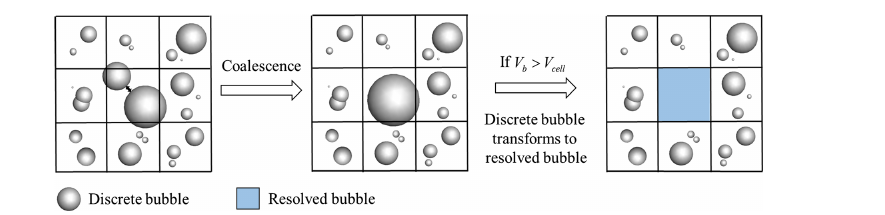
\includegraphics[width=0.93\textwidth]{fig03.png}
\caption{当 $V_b\ge V_{\mathrm{cell}}$ 时，离散气泡向解析气泡转化的示意图。}
\label{fig:transition1}
\end{figure}

第二类是静止于阳极下方的微气泡被沿阳极底面扫过的大变形气泡吞并。假定离散气泡接触到满足 $0.5\le\alpha_g\le1$ 的大气泡界面时即被吸收（图~\ref{fig:swallowmodel}）。其质量加入连续方程，并更新当前网格单元中的气体速度：
\begin{align}
S_2&=\sum_{i=1}^{n}\rho_gV_{bi},\qquad i=1,2,\ldots,n, \tag{33}\\
\vect u_g'&=\vect u_{gi}+\vect u_{bi}\frac{V_{bi}}{V_{\mathrm{cell}}}. \tag{34}
\end{align}

\begin{figure}[H]\centering
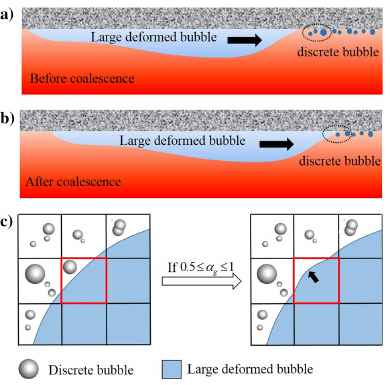
\includegraphics[width=0.62\textwidth]{fig04.png}
\caption{大变形气泡吞并离散气泡的示意图（$0.5\le\alpha_g\le1$）：（a）聚并前；（b）聚并后；（c）转化过程。}
\label{fig:swallowmodel}
\end{figure}

图~\ref{fig:flowchart} 给出了 DBM-VOF 联合算法。两个求解器通过动量交换项 $\vect F_{\mathrm{me}}$ 实现双向耦合，所有方程采用相同时间步推进。计算包含离散气泡聚并和离散-连续转化两个模块。初始离散气泡由 DBM 跟踪，随后通过生长和聚并变大；一旦满足 $V_b\ge V_{\mathrm{cell}}$ 或 $0.5\le\alpha_g\le1$，即转化为 VOF 解析气泡。

\begin{figure}[H]\centering
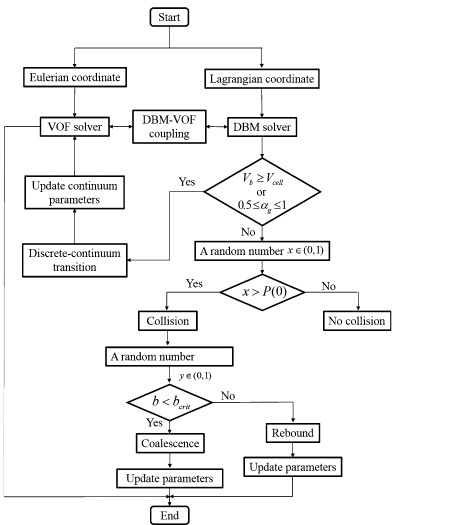
\includegraphics[height=0.62\textheight]{fig05.png}
\caption{DBM-VOF 联合算法流程图。}
\label{fig:flowchart}
\end{figure}

\section{数值细节}

本文采用基于有限体积法的 Fluent 15.0，并通过 UDF 实现模型。计算域采用六面体网格（图~\ref{fig:mesh}），几何与物性参数见表~\ref{tab:param}。

\begin{figure}[H]\centering
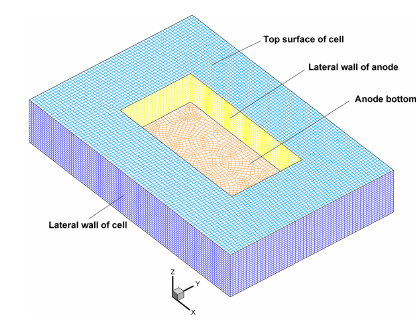
\includegraphics[width=0.68\textwidth]{fig06.png}
\caption{计算网格。}
\label{fig:mesh}
\end{figure}

\begin{table}[H]\centering
\caption{几何参数和物性参数。}
\label{tab:param}
\begin{tabular}{ll}
\toprule
参数 & 数值\\
\midrule
电流密度 & $9000~\mathrm{A/m^2}$\\
阳极底面 & $22\times50~\mathrm{mm}$\\
电解槽 & $90\times60\times20~\mathrm{mm}$\\
\multicolumn{2}{l}{\textit{电解质物性}}\\
密度 & $2130~\mathrm{kg/m^3}$\\
动力黏度 & $0.002513~\mathrm{kg/(m\,s)}$\\
\multicolumn{2}{l}{\textit{气体物性}}\\
密度 & $0.398~\mathrm{kg/m^3}$\\
动力黏度 & $0.00005~\mathrm{kg/(m\,s)}$\\
表面张力 & $0.12~\mathrm{N/m}$\\
\bottomrule
\end{tabular}
\end{table}

网格无关性研究采用 362000、198000 和 134000 个网格单元。第一套与第二套网格所得平均速度相差约 2.4\%，第二套与第三套相差约 3.9\%。综合计算时间和精度，最终采用 198000 个网格单元，典型网格尺寸约为 0.8 mm（图~\ref{fig:grid}）。

\begin{figure}[H]\centering
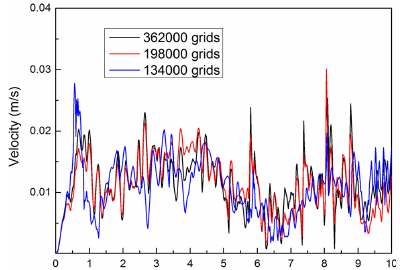
\includegraphics[width=0.72\textwidth]{fig07.png}
\caption{网格数量对点 $(30,0,7~\mathrm{mm})$ 速度的影响。}
\label{fig:grid}
\end{figure}

阳极底面为离散微气泡速度入口；槽顶为出流边界并施加零剪切应力；阳极侧壁、槽侧壁和槽底均为无滑移壁面。初始气泡直径取 0.5 mm，这是若干实验\([11,13,14]\)中观察到的最小气泡尺度。气泡按式（11）生长；当生长或聚并后的体积大于单元体积时，通过 UDF 由离散微气泡转化为解析气泡。

Zhao 等\([13]\)的实验未表现出明显湍流特征，因此采用瞬态层流模型计算低雷诺数气泡-电解质两相流。气液压力-速度耦合采用相耦合 SIMPLE 算法；体积分数瞬态离散采用有界二阶格式。流动时间步为 $10^{-4}$ s，收敛判据为 $10^{-6}$。

\section{结果与讨论}

\subsection{模型验证}

图~\ref{fig:validation} 比较了考虑微观和宏观气泡后，气泡覆盖率及气泡层厚度的实验值与模拟值。通过逐时间步跟踪微气泡轨迹和解析宏观气泡表面，计算平均气泡厚度和覆盖率。两组结果及其波动频率均吻合良好，说明本模型适合预测铝电解槽内的气泡覆盖率和厚度。

\begin{figure}[H]\centering
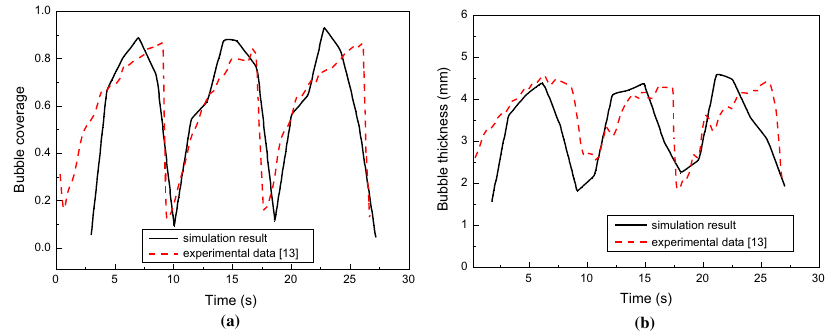
\includegraphics[width=0.94\textwidth]{fig08.png}
\caption{电流密度为 $9000~\mathrm{A/m^2}$ 时实验与模拟结果比较：（a）气泡覆盖率；（b）气泡层厚度。}
\label{fig:validation}
\end{figure}

\subsection{离散气泡聚并}

在气泡初始生长阶段，离散微气泡近似球形。图~\ref{fig:microcoal} 展示了连续的微气泡聚并过程：两个微气泡在阳极下运动时先发生碰撞，随后聚并为大气泡。新气泡体积等于两个小气泡体积之和，其速度按式（20）更新。

\begin{figure}[H]\centering
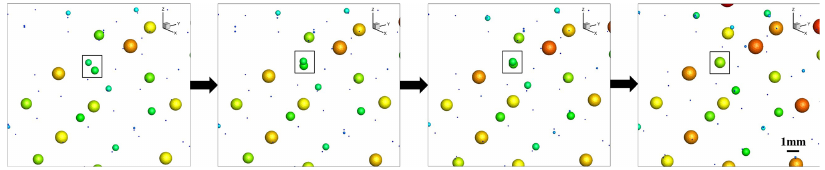
\includegraphics[width=0.96\textwidth]{fig09.png}
\caption{离散气泡聚并过程。}
\label{fig:microcoal}
\end{figure}

\subsection{离散-连续转化}

图~\ref{fig:dct} 展示了离散-连续转化。图（a）中，DBM 在拉格朗日框架下跟踪气泡并逐时间步更新其尺寸和位置；当 $V_b\ge V_{\mathrm{cell}}$ 时，在气泡中心所在位置完成转化，随后由欧拉网格解析气泡界面，如图（b）所示。

\begin{figure}[H]\centering
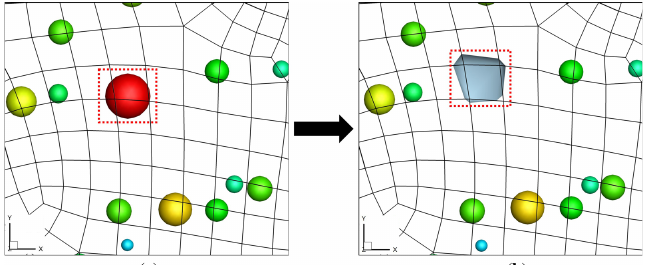
\includegraphics[width=0.76\textwidth]{fig10.png}
\caption{当 $V_b\ge V_{\mathrm{cell}}$ 时的离散-连续转化：（a）转化前；（b）转化后。}
\label{fig:dct}
\end{figure}

图~\ref{fig:swallow} 给出大解析气泡吞并离散微气泡的现象。当离散气泡到达 $0.5\le\alpha_g\le1$ 的界面区域时被吸收，同时更新解析气泡的质量和速度。

\begin{figure}[H]\centering
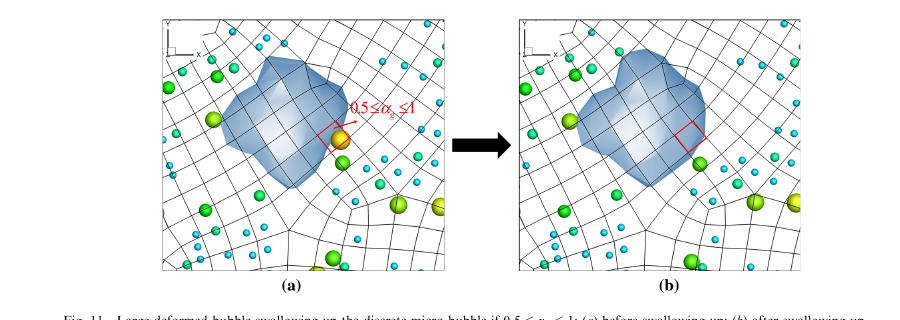
\includegraphics[width=0.84\textwidth]{fig11.png}
\caption{当 $0.5\le\alpha_g\le1$ 时，大变形气泡吞并离散微气泡：（a）吞并前；（b）吞并后。}
\label{fig:swallow}
\end{figure}

\subsection{大变形气泡聚并}

图~\ref{fig:largecoal} 显示模拟得到的大气泡聚并过程，同时可见微气泡与大气泡共存。微气泡转化为大气泡后，在浮力、表面张力和压力梯度力作用下发生变形；大气泡还能吸收附近的离散气泡而继续增大。模型再现了实验\([13,14]\)所区分的六类聚并：小-小（S-S）、中-小（M-S）、中-中（M-M）、大-小（L-S）、大-中（L-M）和大-大（L-L）聚并，说明模型能够有效揭示大气泡聚并过程。

\begin{figure}[H]\centering
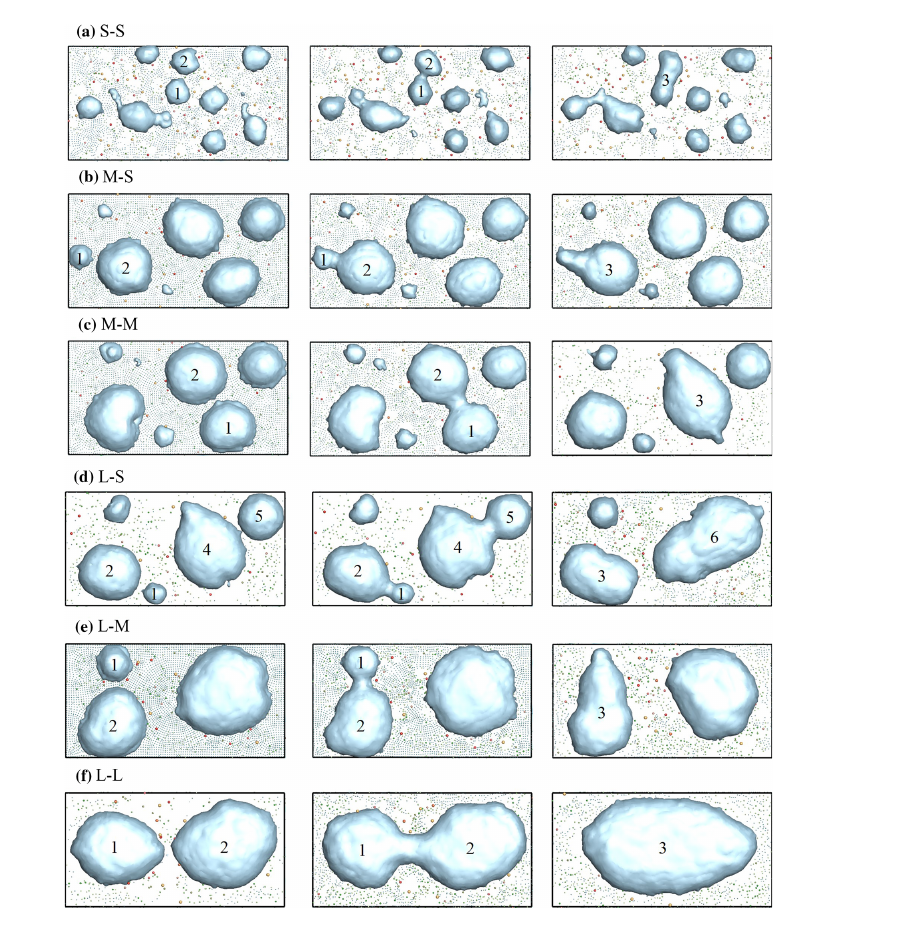
\includegraphics[width=0.90\textwidth,height=0.70\textheight,keepaspectratio]{fig12.png}
\caption{大气泡聚并过程：（a）S-S；（b）M-S；（c）M-M；（d）L-S；（e）L-M；（f）L-L。}
\label{fig:largecoal}
\end{figure}

\subsection{气泡覆盖率与释放频率}

图~\ref{fig:frequencyseries} 给出了不同电流密度下 0--60 s 内的气体覆盖率和气泡释放频率。锯齿状波形反映气泡的生成、生长和脱离；幅值最大的频率峰对应气泡从阳极底面脱离。电流密度由 $1000~\mathrm{A/m^2}$ 增至 $10000~\mathrm{A/m^2}$ 时，气泡释放频率由 0.035 Hz 增至 0.196 Hz。较高电流加快电化学反应，从而提高气泡生成和生长速率，使气泡更快达到释放临界状态；驻留时间缩短，限制了大气泡形成，故释放气泡尺寸更小。最大气体覆盖率也随电流密度升高略有下降，这有利于增大阳极底面与熔融电解质的接触面积并提高电导率。

\begin{figure}[H]\centering
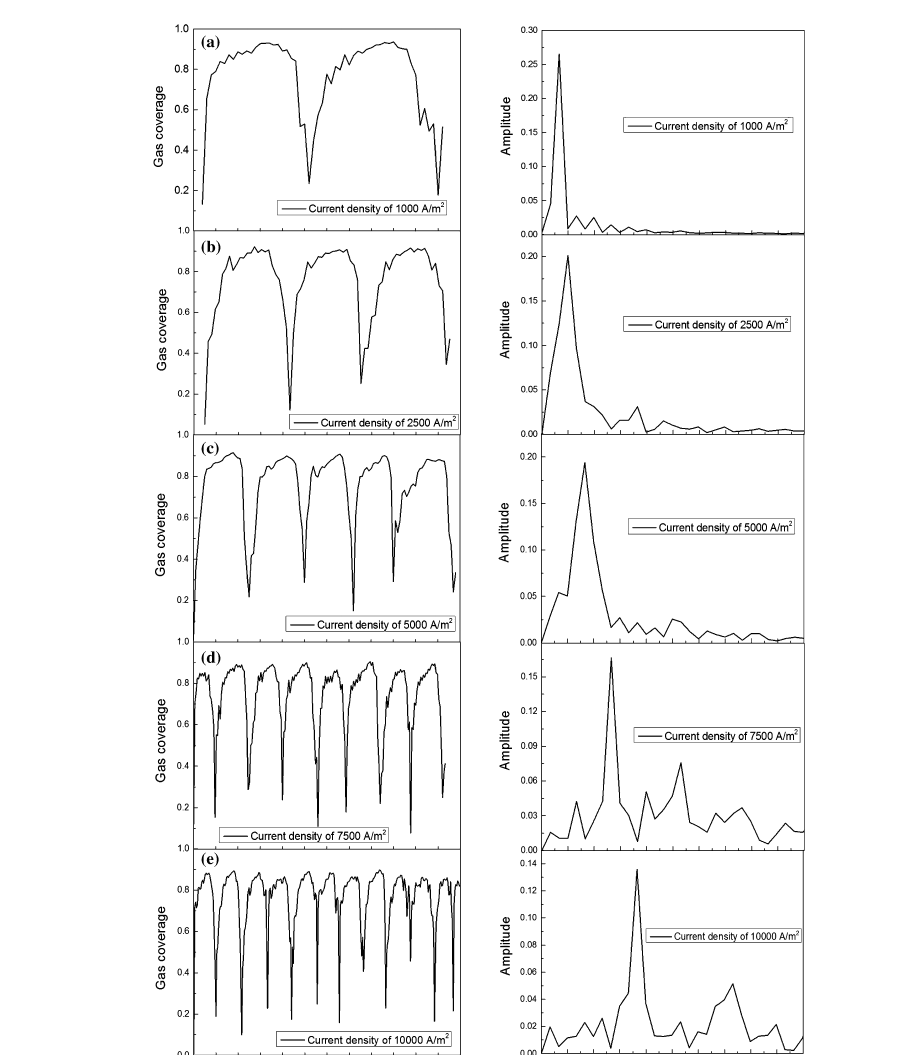
\includegraphics[height=0.70\textheight]{fig13.png}
\caption{不同电流密度下的气体覆盖率和气泡释放频率：（a）1000；（b）2500；（c）5000；（d）7500；（e）$10000~\mathrm{A/m^2}$。}
\label{fig:frequencyseries}
\end{figure}

图~\ref{fig:frequency} 表明释放频率随电流密度增加而上升。Xue\([11]\)实验的阳极小于 Zhao 等\([13]\)所用阳极，因而气泡驻留时间更短、释放频率更高。本文按 Zhao 的实验模型在室温下计算，并假定阳极润湿性不随温度改变，电解质-阳极接触角取 $90^\circ$；实验接触角约为 $100^\circ$--$120^\circ$。较小的接触角意味着润湿性更好\([13]\)，会减小气泡沿竖直表面的上升距离并提高释放频率。

\begin{figure}[H]\centering
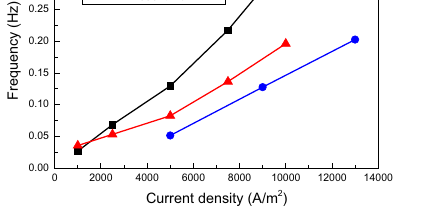
\includegraphics[width=0.72\textwidth]{fig14.png}
\caption{气泡释放频率随电流密度的变化。}
\label{fig:frequency}
\end{figure}

\subsection{气泡厚度}

图~\ref{fig:thickness} 展示气泡厚度的演化。气泡继续生长时由球形转为椭球形，主要原因是垂直于阳极底面的浮力使气泡扁平化。聚并发生时气泡厚度增大、数量减少；达到特定厚度后，气泡开始沿阳极底面铺展，厚度不再增长。最大厚度约 4.2 mm，与已有观察\([8,13,14,18,47,48]\)一致。体积足够大时形成 Fortin 气泡。由于阳极底面水平，气泡由阳极中心向两侧边缘铺展，形成两个厚头部，而倾斜阳极实验中常见的单厚头和细尾并不明显。尽管几何体系对称，气泡运动仍具有随机性；不同尺寸气泡之间的聚并以及碰撞后的速度差异造成了不对称分布。

\begin{figure}[H]\centering
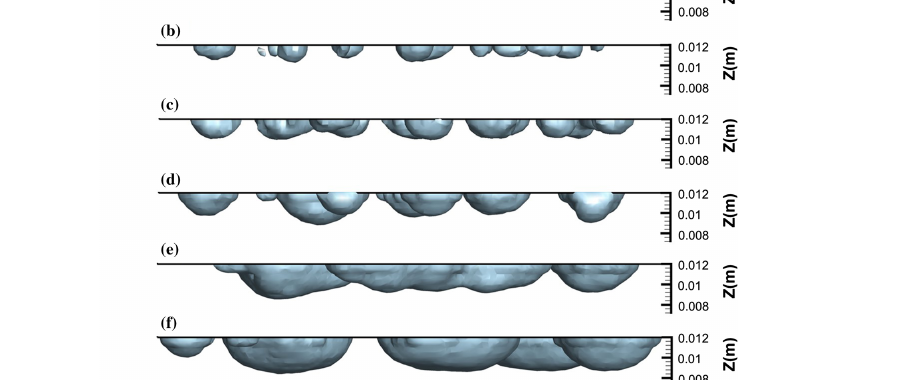
\includegraphics[width=0.96\textwidth]{fig15.png}
\caption{气泡厚度演化：（a）2.5 s；（b）3.1 s；（c）3.7 s；（d）4.3 s；（e）4.9 s；（f）5.5 s；（g）6.1 s；（h）6.7 s。}
\label{fig:thickness}
\end{figure}

图~\ref{fig:thicknesscurrent} 给出最大和平均气泡厚度随电流密度的变化。电流密度为 $7500~\mathrm{A/m^2}$ 时最大厚度达到 4.55 mm，之后随电流密度升高而减小。考虑微气泡和宏观气泡后，平均厚度始终随电流密度升高而下降；微气泡对整体厚度影响很小。高电流通过提高释放频率降低气泡厚度，可能减弱气泡动力学对熔融电解质的影响，并允许缩短 ACD、降低能耗。

\begin{figure}[H]\centering
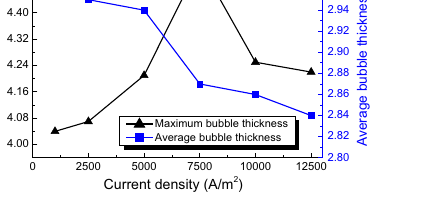
\includegraphics[width=0.72\textwidth]{fig16.png}
\caption{最大和平均气泡厚度随电流密度的变化。}
\label{fig:thicknesscurrent}
\end{figure}

\section{结论}

本文建立了带离散-连续转化的三维 DBM-VOF 模型，用于预测铝电解槽内的气泡-电解质两相流。离散微气泡由 DBM 描述，大气泡由 VOF 在宏观尺度上完整解析，并利用 UDF 实现新的离散气泡向大气泡转化。主要结论如下：

\begin{enumerate}[label=\arabic*.]
\item 模型实现了三类气泡聚并：DBM 描述离散微气泡之间的聚并；DBM 与 VOF 耦合描述大变形气泡吞并离散气泡；VOF 解析大气泡之间的聚并。
\item 气泡聚并时厚度增加而数量减少；达到特定厚度后，气泡沿阳极底面铺展并停止增厚。水平阳极下可观察到两个厚头部，而细尾不明显。
\item 随电流密度升高，气泡释放频率增大、气体覆盖率降低，释放气泡尺寸减小，阳极-电解质接触面积因而增大，有利于提高电解槽导电性。电流密度对气泡厚度影响较小，本文所得厚度为 4.0--4.5 mm。气体覆盖率和气泡层厚度均与 Zhao 等\([13,14]\)的实验数据吻合良好。
\end{enumerate}

\section*{致谢}

作者感谢复杂有色金属资源清洁利用国家重点实验室开放基金（CNMRCUKF1607）的支持。

\section*{符号说明}

\begin{longtable}{p{0.18\textwidth}p{0.74\textwidth}}
$m_b$ & 气泡质量\\
$m_1',m_1,m_2$ & 聚并后的新气泡质量、大气泡质量、小气泡质量\\
$\vect u_b,\vect u_b'$ & 气泡速度、聚并后的新气泡速度\\
$\vect u_{b1},\vect u_{b2}$ & 大气泡速度、小气泡速度\\
$\vect u_{b1}',\vect u_{b2}'$ & 回弹后大气泡速度、小气泡速度\\
$\vect u_g,\vect u$ & 解析气泡速度、电解质速度\\
$\vect u_{\mathrm{rel}}$ & 相对速度\\
$\vect F_b$ & 浮力与重力合力\\
$\vect F_d,\vect F_{\mathrm{vir}},\vect F_p$ & 曳力、虚质量力、压力梯度力\\
$\vect F_{\mathrm{me}},\vect F_s$ & 动量交换项、表面张力\\
$V_b,V_{\mathrm{cell}}$ & 气泡体积、网格单元体积\\
$d_b,\bar d$ & 气泡直径、两气泡算术平均直径\\
$r,r_1,r_2$ & 气泡半径、大气泡半径、小气泡半径\\
$C_D$ & 曳力系数\\
$I,F,R$ & 电流、法拉第常数、摩尔气体常数\\
$p_1,H,\Delta t$ & 电解质中的气泡压力、阳极浸入深度、时间步\\
$P,N,\bar N,N_1,N_c$ & 碰撞概率、气泡总数、平均碰撞数、小气泡数、碰撞次数\\
$x,y$ & $(0,1)$ 内随机数\\
$b,b_{\mathrm{crit}}$ & 实际碰撞偏心距、临界偏心距\\
$We$ & 碰撞 Weber 数\\
$S_1,S_2$ & 质量源项\\
$\rho,\rho_b,\rho_g,\rho_l$ & 混合物密度、气泡密度、解析气泡密度、电解质密度\\
$\mu,\mu_l,\mu_g$ & 混合物黏度、电解质黏度、解析气泡黏度\\
$\sigma_{ij}$ & 表面张力系数\\
$\kappa$ & 曲率\\
$\alpha,\alpha_g$ & 体积分数、气相体积分数\\
\end{longtable}

\section*{参考文献}
\small
\begin{enumerate}[label={[\arabic*]},leftmargin=2.8em,itemsep=0.15em]
\item S. Fortin, M. Gerhardt, and A.J. Gesing, \emph{Light Metals}, TMS, 1984, pp. 385--395.
\item K. V\'ekony and L.I. Kiss, \emph{Metall. Mater. Trans. B}, 2010, 41B, 1006--1017.
\item A.J. Simonsen, K.E. Einarsrud, and I. Eick, \emph{Light Metals}, 2015, 795--800.
\item M. Alam et al., \emph{Metall. Mater. Trans. B}, 2013, 44B, 1155--1165.
\item A.L. Perron, L.I. Kiss, and S. Poncs\'ak, \emph{Int. J. Multiph. Flow}, 2006, 32, 1311--1325.
\item A.L. Perron, L.I. Kiss, and S. Poncs\'ak, \emph{Int. J. Multiph. Flow}, 2006, 32, 606--622.
\item L.I. Kiss et al., \emph{Multiphase Phenomena and CFD Modeling and Simulation in Materials Processes}, 2004, 159--168.
\item S. Das et al., \emph{Colloids Surf. A}, 2012, 411, 94--104.
\item S. Das, L.D. Weerasiri, and W. Yang, \emph{Colloids Surf. A}, 2017, 516, 23--31.
\item Z.B. Zhao et al., \emph{Metall. Mater. Trans. B}, 2017, 48B, 1200--1216.
\item J.L. Xue and A.O. Oye, \emph{Light Metals}, 1995, 265--271.
\item L. Cassayre, T.A. Utigard, and S. Bouvet, \emph{JOM}, 2002, 54, 41--45.
\item Z. Zhao et al., \emph{JOM}, 2017, 69, 281--291.
\item Z. Zhao et al., \emph{Metall. Mater. Trans. B}, 2016, 47B, 1962--1975.
\item Z. Qiu et al., \emph{J. Appl. Electrochem.}, 1987, 17, 707--714.
\item Z. Qiu and M. Zhang, \emph{Electrochim. Acta}, 1987, 32, 607--613.
\item W.E. Haupin and W.C. McGrew, \emph{Light Metals}, 1974, 37--47.
\item T. Utigard and J.M. Toguri, \emph{Light Metals}, 1986, 405--413.
\item R. Keller and K.T. Larimer, \emph{Light Metals}, 1992, 464--467.
\item Z. Zhao et al., \emph{Light Metals}, 2015, 801--806.
\item S. Poncsak, L.I. Kiss, and R.T. Bui, 38th Annual Meeting of CIM, Qu\'ebec, 1999.
\item A.L. Perron, L.K. Kiss, and S. Poncsak, \emph{J. Appl. Electrochem.}, 2006, 36, 1381--1389.
\item A.L. Perron, L.K. Kiss, and S. Poncsak, \emph{J. Appl. Electrochem.}, 2007, 37, 303--310.
\item Y.F. Wang, L.F. Zhang, and X.J. Zuo, \emph{Metall. Mater. Trans. B}, 2011, 42B, 1051--1064.
\item A. Caboussat et al., \emph{Light Metals}, 2011, 581--586.
\item K. Zhang et al., \emph{J. Appl. Electrochem.}, 2014, 44, 1081--1092.
\item J. Li et al., \emph{Int. J. Multiph. Flow}, 2011, 37, 46--54.
\item Q. Wang et al., \emph{Metall. Mater. Trans. B}, 2014, 45B, 272--294.
\item Y. Feng et al., \emph{Metall. Mater. Trans. B}, 2015, 46B, 1959--1981.
\item S.Q. Zhan et al., \emph{J. Cent. South Univ.}, 2015, 22, 2482--2492.
\item K.E. Einarsrud et al., \emph{Appl. Math. Model.}, 2017, 44, 3--24.
\item S. Poncsak, L.K. Kiss, and D. Toulouse, \emph{Light Metals}, 2006, 457--462.
\item S. Zhan et al., \emph{Light Metals}, 2014, 777--782.
\item L. Li et al., \emph{ISIJ Int.}, 2015, 55, 1337--1346.
\item M. Sun et al., \emph{Metall. Mater. Trans. B}, 2017, 48B, 3161--3173.
\item \emph{ANSYS Fluent User Manual}, ANSYS Inc., 2015.
\item E.I.V.V.D. Hengel, N.G. Deen, and J.A.M. Kuipers, \emph{Ind. Eng. Chem. Res.}, 2005, 44, 5233--5245.
\item L.M. Li and B.K. Li, \emph{JOM}, 2016, 68, 2160--2169.
\item S.A. Morsi and A.J. Alexander, \emph{J. Fluid Mech.}, 1972, 55, 193--208.
\item J. Zhang, Y. Li, and L. Fan, \emph{Powder Technol.}, 2000, 112, 46--56.
\item L. Li and B. Li, \emph{Particuology}, 2018, 39, 109--115.
\item P.J. O'Rourke, Ph.D. thesis, Princeton University, 1981.
\item J. Zhang, J. Mi, and H. Wang, \emph{Aerosol Sci. Technol.}, 2012, 46, 622--630.
\item C.W. Hirt and B.D. Nichols, \emph{J. Comput. Phys.}, 1981, 39, 201--225.
\item A. Jardy, D. Ablitzer, and J.F. Wadier, \emph{Metall. Mater. Trans. B}, 1991, 22B, 111--120.
\item J.U. Brackbill, D.B. Kothe, and C. Zemach, \emph{J. Comput. Phys.}, 1992, 100, 335--354.
\item T. Utigard, J.M. Toguri, and S.W. Ip, \emph{Light Metals}, 1988, 703--706.
\item Z. Qiu, \emph{Principle and Application of Aluminum Electrolysis}, China University of Mining and Technology Press, 1998, p. 572.
\end{enumerate}

\vfill
\begin{center}\footnotesize 翻译依据：Sun, Li and Li, \emph{Metallurgical and Materials Transactions B} (2018), DOI: 10.1007/s11663-018-1311-y。\end{center}
\end{document}
